%%%%%%%%%%%%%%%%%%%%%%%%%%%%%%%%%%%%%%%%%%%%%%%%%%%%%%%%%%%%%%%%%%%%%%%%%%%%%%%%%%%%%%%%%%%%%%%%%%%
%%%%%%%%%%%%%%%%%%%%%%%%%%%%%%%%%%%%%%%%%%%%%%%%%%%%%%%%%%%%%%%%%%%%%%%%%%%%%%%%%%%%%%%%%%%%%%%%%%%
%%%%%%%%%%%%%%%%%%%%%%%%%%%%%%%%%%%%%%%%%%%%%%%%%%%%%%%%%%%%%%%%%%%%%%%%%%%%%%%%%%%%%%%%%%%%%%%%%%%

\chapter{Resultados}

Previo al análisis de la estacionariedad, se corroboró la hipótesis de que las variables 
independientes son estadísticamente iguales entre los grupos CTL y PDC. Las comparaciones
usando la prueba $t$ de Welch (cuadro \ref{var_ind}) indican que efectivamente la hipótesis se cumple salvo
para los puntajes de Neuropsi.

Se evalúo si pudieran existir relaciones entre las variables que se presumen independientes.
Usando la prueba de correlación de Spearman (cuadro \ref{cor_ind}) se encontró sólo hay 
correlaciones monotónicas entre los siguientes pares de variables:
\begin{itemize}
\item Edad y Escolaridad
\item Puntaje en Neuropsi y Puntaje en Mini Mental-State Examination (MMSE)
\item Tiempo de MOR (en segundos) y Tiempo en MOR (porcentaje)
\end{itemize}

La primera relación, no muy fuerte, puede explicarse como un \textit{efecto generacional}: la educación 
superior ha aumentado su cobertura durante las últimas décadas, y entonces los grupos poblacionales 
más jóvenes tienen en promedio más años de escolaridad. 
%
Algunos autores han sugerido que un bajo nivel de escolaridad es un factor de riesgo para padecer
deterioro cognitivo, en base a estudios horizontales de larga escala \cite{Mejia_Arango2007}.
%
En el presente trabajo se ignora este dato, en vista de que no se pudieron relacionar el nivel de 
escolaridad de los participantes con su desempeño en pruebas neuropsicológicas.

La relación entre los puntajes en Neuropsi y en MMSE era de esperarse, ya que ambas pruebas miden
parámetros similares y tienen contenidos independientes. Cabe mencionar el curioso fenómeno en que (1) 
los puntajes de MMSE
tienen estadísticamente las mismas medias grupales, (2) los puntajes de MMSE están 
fuertemente correlacionados con los puntajes de Neuropsi, y (3) los puntajes de Neuropsi
tienen estadísticamente medias grupales diferentes. Se confirma que la prueba MMSE
tiene menor sensibilidad que la prueba Neuropsi para detectar deterioro cognitivo.

Era por demás obvia la relación entre la cantidad total de sueño MOR, con su proporción respecto a 
todo el sueño. Sin embargo, conviene mencionar que la cantidad de sueño MOR no es afectada por
ninguna de las otras variables independientes; luego entonces las cantidades que fueron estudiadas
(estacionariedad, espectro de potencias) no tienen correlaciones sesgadas con las demás variables.

\begin{table}
\centering
\caption{Variables independientes entre grupos}
\begin{tabular}{lrlcrlcccc}
\toprule
 & \multicolumn{2}{l}{Grupo CTL} & \phantom{.} & \multicolumn{2}{l}{Grupo PDC} 
 & \phantom{.} & \multicolumn{3}{l}{t de Welch}
 \\
\cmidrule{2-3} \cmidrule{5-6} \cmidrule{8-10}
& Media & (DE) & & Media & (DE) & & $p$ & $t$ & $\nu$ \\
\midrule
Edad              &  68.2   & (7.2)     & &    67.6 & (3.4)     & & 0.8746 & 0.16 & 6.11 \\
Escolaridad       &   9.2   & (2.7)     & &     8.4 & (2.2)     & & 0.6201 & 0.52 & 7.69 \\
Neuropsi          & 108.9   & (5.2)     & &    87.8 & (5.6)     & & \bf 0.0003 & 6.17 & 7.94 \\
MMSE              &  29.4   & (0.9)     & &    27.4 & (1.4)     & & 0.0706 & 0.16 & 6.11 \\
Sueño [s]         & 7:51:30 & (0:57:36) & & 7:16:48 & (2:24:43) & & 0.6836 & 0.50 & 5.24 \\
MOR [s]           & 0:52:06 & (0:23:00) & & 0:34:18 & (0:22:14) & & 0.2486 & 1.24 & 7.99 \\
MOR [\%]          &  11.3   & (5.1)     & &     8.4 & (4.8)     & & 0.3871 & 0.91 & 7.96 \\
\bottomrule 
\multicolumn{5}{l}{DE=Desviación Estándar}
\end{tabular} 
\label{var_ind}
\end{table}

\begin{table}
\centering
\caption{Correlaciones entre variables independientes}
\begin{tabular}{llllllll}
\toprule
  &             & 1 & 2 & 3 & 4 & 5 & 6 \\
\midrule
1 & Edad        & $\bullet$  &          &           &          &          & \\
2 & Escolaridad & -0.7134* &  $\bullet$ &           &          &          & \\
3 & Neuropsi    & -0.2432  & \phm 0.3776  & $\bullet$   &          &          & \\
4 & MMSE        & -0.1063  & \phm 0.1812  & 0.8477*** & $\bullet$  &          & \\
5 & Sueño [s]   & \phm  0.0486  & -0.0944  & 0.0545    & 0.0374   & $\bullet$  & \\
6 & MOR [s]     & \phm 0.2796  & -0.5035  & 0.1879    & 0.2618   & -0.1515  & $\bullet$ \\
7 & MOR [\%]    & \phm 0.3709  & -0.5287  & 0.0182    & 0.0748   & -0.3578  & 1**** \\
\bottomrule
\multicolumn{7}{l}{Niveles de significancia: *$<$.05 , **$<$.01 , ***$<$.005 , ****$<$.001}
\end{tabular}
\label{cor_ind}
\end{table}

%%%%%%%%%%%%%%%%%%%%%%%%%%%%%%%%%%%%%%%%%%%%%%%%%%%%%%%%%%%%%%%%%%%%%%%%%%%%%%%%%%%%%%%%%%%%%%%%%%%
%%%%%%%%%%%%%%%%%%%%%%%%%%%%%%%%%%%%%%%%%%%%%%%%%%%%%%%%%%%%%%%%%%%%%%%%%%%%%%%%%%%%%%%%%%%%%%%%%%%

\section{Estacionariedad en sueño MOR}

Se sometió a prueba la hipótesis de que durante sueño MOR ocurre en mayor medida la estacionariedad
débil, en comparación con el sueño NMOR. Para ello, se compararon el porcentaje de épocas 
estacionarias en el sentido de PSR, ocurridas durante sueño MOR y NMOR. La comparación fue efectuada
usando la prueba $\chi^{2}$ de Pearson. Se encontró
de manera consistente que los canales ROG y LOG presentaron diferencias significativas ($p<0.05$) 
entre sueño MOR y NMOR, lo cual puede explicarse por los movimientos oculares rápidos característicos
del sueño MOR. En los canales que corresponden al EEG no se encontraron patrones consistentes y 
claros entre los sujeto (ver figura \ref{cabeza_new}).

\begin{figure}
\centering
\begin{tabular}{ccccc}
VCR & MJH & JAE & GHA & MFGR \\
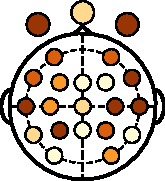
\includegraphics[width=0.17\textwidth]{./img_art_dfa/cabeza_new_VCR_30.pdf} &
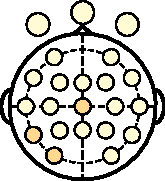
\includegraphics[width=0.17\textwidth]{./img_art_dfa/cabeza_new_MJH_30.pdf} &
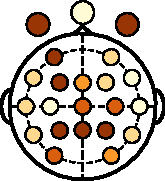
\includegraphics[width=0.17\textwidth]{./img_art_dfa/cabeza_new_JAE_30.pdf} &
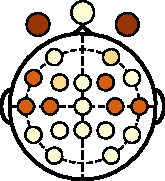
\includegraphics[width=0.17\textwidth]{./img_art_dfa/cabeza_new_GHA_30.pdf} &
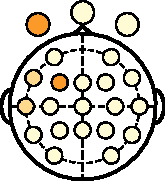
\includegraphics[width=0.17\textwidth]{./img_art_dfa/cabeza_new_MFGR_30.pdf} \\
\midrule
CLO & RLO & RRU & JGZ & AEFP \\
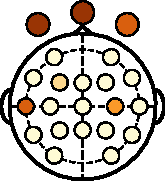
\includegraphics[width=0.17\textwidth]{./img_art_dfa/cabeza_new_CLO_30.pdf} &
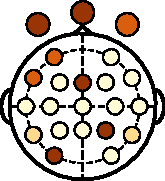
\includegraphics[width=0.17\textwidth]{./img_art_dfa/cabeza_new_RLO_30.pdf} &
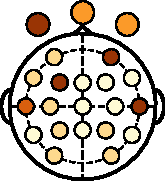
\includegraphics[width=0.17\textwidth]{./img_art_dfa/cabeza_new_RRU_30.pdf} &
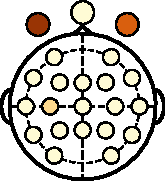
\includegraphics[width=0.17\textwidth]{./img_art_dfa/cabeza_new_JGZ_30.pdf} &
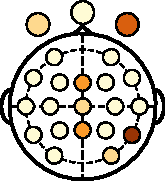
\includegraphics[width=0.17\textwidth]{./img_art_dfa/cabeza_new_AEFP_30.pdf} \\
\end{tabular} \\

\includegraphics[scale=.7]{./img_art_dfa/escala.pdf} \\
\caption{Regiones donde la cantidad de ventanas estacionarias es significativamente diferente 
durante sueño MOR y NMOR, usando ventanas de 30 segundos}
\label{cabeza_new}
\end{figure}

Se repitió la comparación a un nivel grupal, usando la prueba $U$ de  Mann-Whitney.
Se encontraron diferencias significativas para el grupo CTL en los canales P3, P4, PZ, 
ROG y EMG; en el grupo PDC se observaron tales diferencias sólo en P4.
%
Las proporciones muestran tendencias que, quizá, resultaron no ser significativas
por el tamaño pequeño de la muestra: los canales P3 y PZ podrían ser diferentes también para
individuos del grupo PDC, y el canal LOG podría ser diferente durante sueño MOR y NMOR.
%
Así mismo se hipotetiza que para el grupo CTL, en todos los canales, el sueño MOR
es presenta menor cantidad de épocas estacionarias.

Se concluye que
no se puede establecer diferencias entre las medias grupales para esta cantidad (proporción de
épocas estacionarias, medidas en el sentido de PSR), debido a la gran variabilidad entre sujetos.

\begin{figure}
\centering
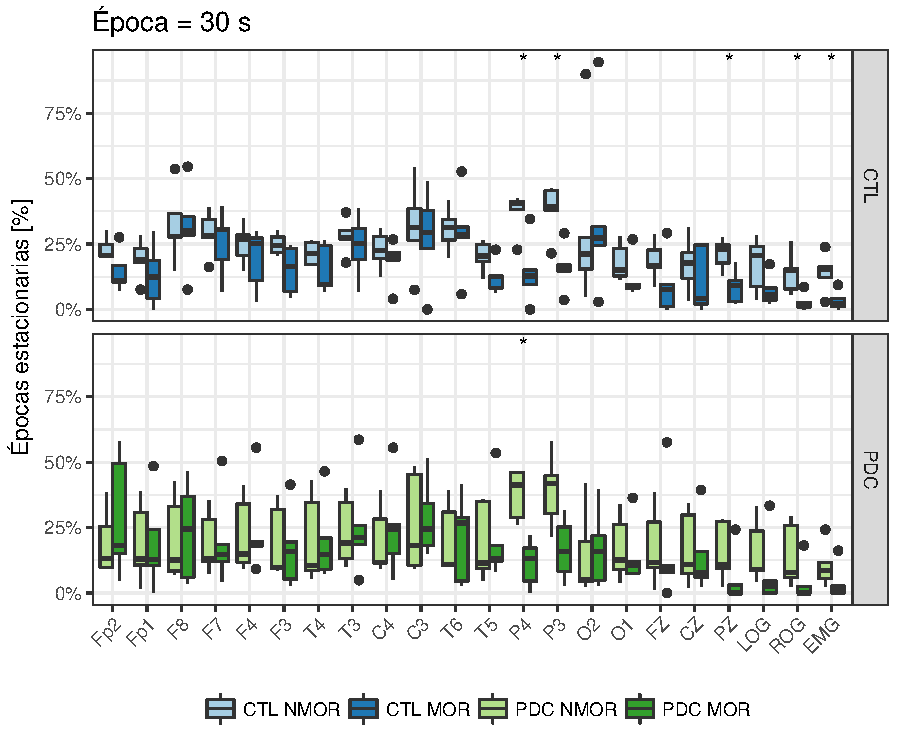
\includegraphics[width=\linewidth]
{./img_art_dfa/Comparacion_gpos_CTL_PDC_v3.pdf}
\caption{Proporciones de épocas estacionarias, durante sueño MOR y NMOR.}
\label{comparacion_verde}
\end{figure}

\begin{figure}
\centering
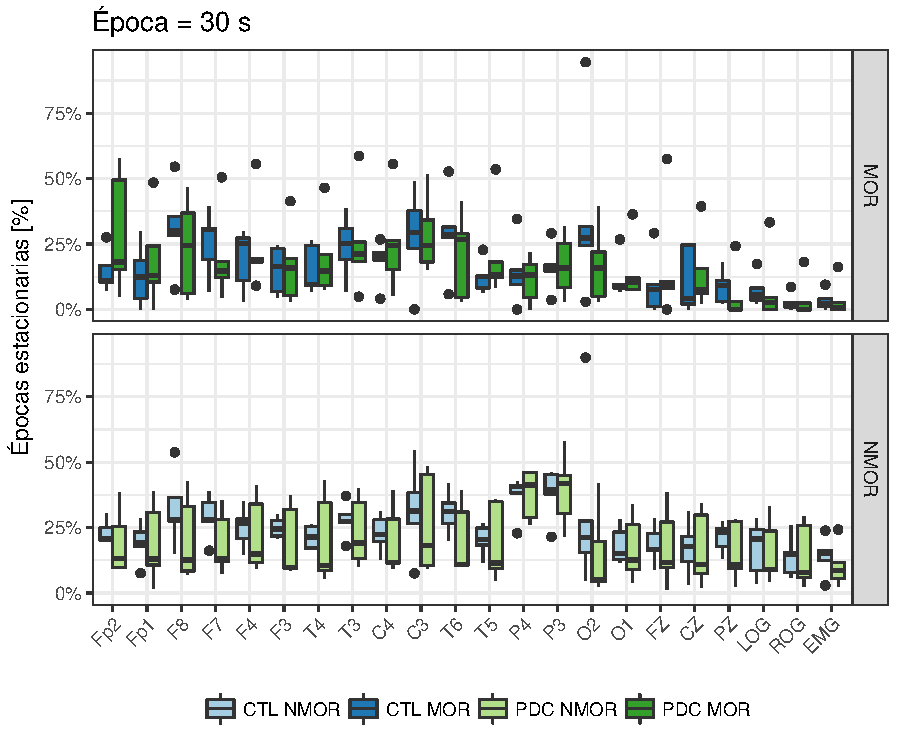
\includegraphics[width=\linewidth]
{./img_art_dfa/Comparacion_gpos_MOR_NMOR_v3.pdf}
\caption{Proporciones de épocas estacionarias, grupos CTL y PDC.}
\label{comparacion_graf}
\end{figure}

%%%%%%%%%%%%%%%%%%%%%%%%%%%%%%%%%%%%%%%%%%%%%%%%%%%%%%%%%%%%%%%%%%%%%%%%%%%%%%%%%%%%%%%%%%%%%%%%%%%
%%%%%%%%%%%%%%%%%%%%%%%%%%%%%%%%%%%%%%%%%%%%%%%%%%%%%%%%%%%%%%%%%%%%%%%%%%%%%%%%%%%%%%%%%%%%%%%%%%%
%%%%%%%%%%%%%%%%%%%%%%%%%%%%%%%%%%%%%%%%%%%%%%%%%%%%%%%%%%%%%%%%%%%%%%%%%%%%%%%%%%%%%%%%%%%%%%%%%%%

\section{Discusión}

%Una práctica común en el análisis de señales electrofisiológicas es el suponer que una serie de 
%tiempo \textit{suficientemente} corta pueda considerarse estacionaria, cuando menos en el sentido
%débil; anteriormente se ha señalado que se trata de un efecto de muestras pequeñas \cite{Melard89},
%y paralelamente se han incorporado a los diseños experimentales motivos para mantener este supuesto
%\cite{Kaiser00}.
%
%Este trabajo parte de la hipótesis de que adultos mayores con PDC presentan en mayor medida 
%estacionariedad débil en sus registros de PSG; al comparar sujetos de los grupo Nn (control) y Mn 
%(PDC), no se observaron cambios significativos en la porción de tiempo durante la cual el registro 
%de PSG se comporta como débilmente estacionario. 
%Esto puede interpretarse como que los cambios en la corteza cerebral durante el deterioro 
%cognitivo, no provocan que  la señal se vuelva más \textit{simple} en el sentido de 
%\textit{volverse} estacionaria.
%
%Comparando grupalmente la cantidad de épocas estacionarias durante MOR y NMOR, se encontró que en 
%el grupo Nn había diferencias significativas en sitios de la región frontal y que no eran presentes
%en el grupo Mn; para poder establecer una relación con el PDC haría falta un mayor grupo muestral, 
%o bien nuevos registros de PSG para los mismos sujetos, o incluso analizar registros de EEG durante 
%otro tipo de actividades y confirmar las diferencias encontradas.
%
%Cabe destacar que la evidencia aportada indica que el PSG es un conjunto de señales que se comportan
%como no-estacionarias durante la mayor parte del sueño, lo cual confirma el supuesto usual de que 
%las señales de origen biológico son por naturaleza no-estacionarias. 

%\subsection{Efecto del tamaño de las época}

%En el apéndice X se explica que si disminuye el tamaño de época el test de PSR disminuye su 
%potencia, de modo que es más propensa a dar falsos negativos (rechazar la hipótesis de 
%estacionariedad cuando debía aceptarse); entonces, en épocas más pequeñas debería haber más épocas 
%clasificadas como no-estacionarias.
%Sin embargo, al \textit{graficar} la estacionariedad para diferentes tamaños de época (figura
%\ref{comp_VCR}) ocurre que es más frecuente el efecto contrario.
%
%\begin{figure}
%\centering
%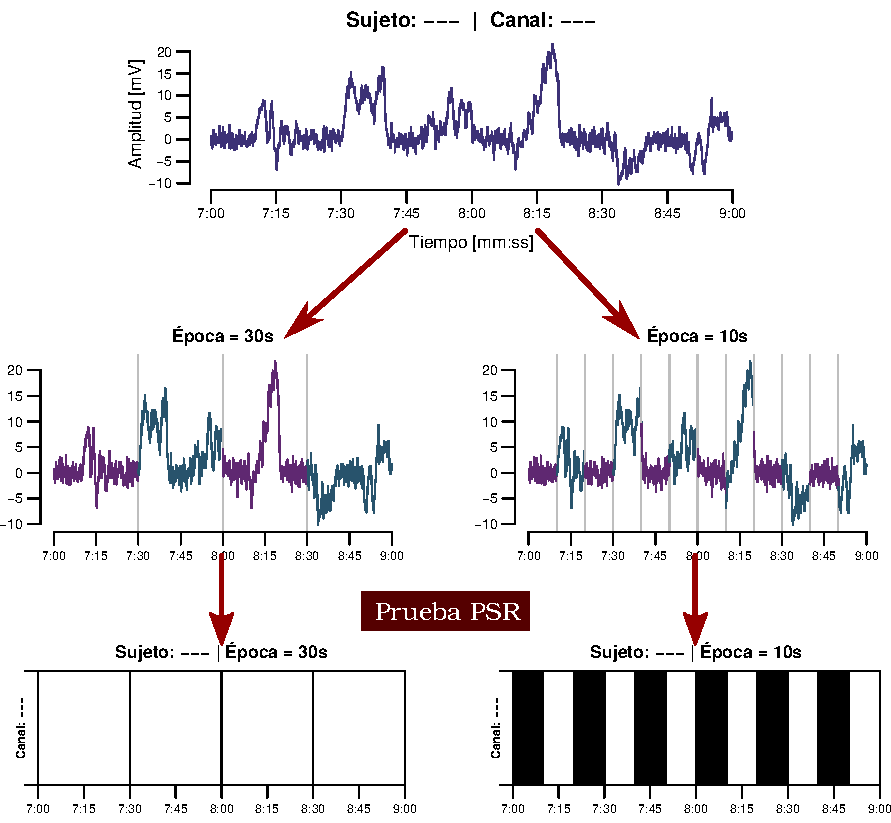
\includegraphics[width=\linewidth]{./img_diagramas/epocas_diferentes_v2.pdf}
%\caption{Efecto del tamaño de ventana sobre la clasificación de estacionariedad}
%\label{epocas_diferentes}
%\end{figure}
%
%Se propone que este efecto puede ser explicado si los registros de PSG son \textbf{localmente
%estacionarios}, una propiedad introducida por Dahlhaus \cite{Dahlhaus97} y que consiste en que un
%proceso no-estacionario pueda ser aproximado a trozos \textit{ensamblando} procesos estacionarios
%definidos para intervalos pequeños de tiempo.
%Esta caracterización del EEG ha sido usada anteriormente de manera fructífera pero problemática
%[??].
%
%En el contexto particular del presente trabajo, la presencia de estacionariedad local puede ser
%explicada fisiológicamente por el contenido heterogéneo de ritmos cerebrales de las etapas de 
%sueño; como ejemplo, en la etapa N3 aparecen husos de sueño mezcladas con ritmos Alfa, de modo
%que es posible hallar un fragmento de época en sueño N3 con únicamente un tren de ondas Alfa
%o un tren de husos de sueño.
%Este fenómeno es ilustrado de manera esquemática en la figura \ref{epocas_diferentes}.
%
%
%
%Entonces, se propone que los registros de PSG se comportan como procesos localmente estacionarios; 
%más aún, se propone que esta característica cambia cualitativamente en adultos mayores con PDC,
%para los cuales el \textit{nivel de homogeneidad} del PSG es muy similar durante MOR y NMOR.

%%%%%%%%%%%%%%%%%%%%%%%%%%%%%%%%%%%%%%%%%%%%%%%%%%%%%%%%%%%%%%%%%%%%%%%%%%%%%%%%%%%%%%%%%%%%%%%%%%%
%%%%%%%%%%%%%%%%%%%%%%%%%%%%%%%%%%%%%%%%%%%%%%%%%%%%%%%%%%%%%%%%%%%%%%%%%%%%%%%%%%%%%%%%%%%%%%%%%%%

\section{Conclusiones}

Se concluye que
es posible la ocurrencia de fragmentos arbitrariamente cortos de registros de PSG que no 
son débilmente estacionarios. Paralelamente, la presencia de estos fragmentos se ve influida por el
estado de actividad del cerebro.
%
Como consecuencia directa de este fenómeno, es posible limitar los efectos \textit{distorsivos} de 
la no-estacionariedad, para lo cual basta un diseño experimental que distinga adecuadamente el
estado de actividad a estudiar. 

En otro ámbito, es en principio posible usar la
proporción de estacionariedad (\textit{densidad} de ventanas estacionarias en el sentido de
PSR) en el EEG para caracterizar estados de actividad cerebral. Para ello, falta 
investigar las características particulares de la etapa que se busca identificar, así como otras
etapas cercanas en el tiempo.

%%%%%%%%%%%%%%%%%%%%%%%%%%%%%%%%%%%%%%%%%%%%%%%%%%%%%%%%%%%%%%%%%%%%%%%%%%%%%%%%%%%%%%%%%%%%%%%%%%%
%%%%%%%%%%%%%%%%%%%%%%%%%%%%%%%%%%%%%%%%%%%%%%%%%%%%%%%%%%%%%%%%%%%%%%%%%%%%%%%%%%%%%%%%%%%%%%%%%%%

\section{Trabajo a futuro}

Una vez que se ha identificado un marcador para el PDC usando un grupo de laboratorio,
conviene automatizar los análisis para su uso clínico sobre un público más general.
%
Un uso más amplio de la técnica asegura una mayor población para poder estudiar la 
efectividad y sensibilidad de la prueba
Y más que eso, se espera que puedan ser sinceramente beneficiosos para los pacientes. Siguiendo el
protocolo usual, los marcadores presentados no serán usados como único recurso para generar
un diagnóstico clínico, sino como un apoyo a las herramientas existentes.

El uso de marcadores basados en registros de PSG --basados en el EEG en general-- aporta una
base fisiológica al diagnóstico de deterioro cognitivo, misma que no es posible usando
únicamente pruebas neuropsicológicas.
%
Conviene destacar que, de entre las herramientas para el registro fisiológico del sistema nervioso
central, las técnicas electrofisiológicas son las más económicas y menos invasivas;
generar marcadores basados en ellas facilita su uso por el público general como herramienta 
diagnóstica, sobre todo en ausencia de síntomas.

%%%%%%%%%%%%%%%%%%%%%%%%%%%%%%%%%%%%%%%%%%%%%%%%%%%%%%%%%%%%%%%%%%%%%%%%%%%%%%%%%%%%%%%%%%%%%%%%%%%
%%%%%%%%%%%%%%%%%%%%%%%%%%%%%%%%%%%%%%%%%%%%%%%%%%%%%%%%%%%%%%%%%%%%%%%%%%%%%%%%%%%%%%%%%%%%%%%%%%%
%%%%%%%%%%%%%%%%%%%%%%%%%%%%%%%%%%%%%%%%%%%%%%%%%%%%%%%%%%%%%%%%%%%%%%%%%%%%%%%%%%%%%%%%%%%%%%%%%%%
